% !TeX root = ../main.tex

\chapter{排序算法加速器的应用——大数据集八叉树构建过程加速}

在本章中,我们将之前的实验结果运用到实际问题——构建大数据集的八叉树过程当中。以此来举例排序算法加速器的可能应用场景。

\section{八叉树简介}






八叉树(Octree)是一种树形的数据结构。其特点在于每个内部结点都有8个子节点。而与此同时,如果在三维直角坐标系中对三维空间进行划分,也可以划分成8个卦限。因此,八叉树经常被用于分割三维空间,通过增加子节点的层级可以将空间无限递归划分\cite{meagher1980octree},如图\ref{fig:octree}所示。显然,在构建八叉树的过程中,我们需要确定空间划分的最小尺度(分辨率),从而设定八叉树的最大递归深度。八叉树的优点在于其能够快速进行空间查询。而空间查询是计算机视觉邻域中一个重要的过程:在碰撞检测的粗检测中需要运用到空间查询;在射击游戏中,需要运用空间查询来进行邻近查询;在光线追踪领域当中,也需要利用空间查询来确定光线的入射位置以及反射方向。

在构建八叉树的过程中,我们常用莫顿码\cite{morton1966computer}来对节点坐标进行编码,其编码方式如图\ref{fig:morton_code}所示。使用莫顿码表示节点坐标有诸多好处。首先,它将三维坐标转化为二进制编码,压缩了空间,且方便了结点的索引;其次,莫顿码的Z字形遍历编码方式使得在空间中相邻的结点具有相近的值,使得其与八叉树具有直接映射的关系($3k$比特的莫顿码映射到八叉树的第$k$层\cite{karras2012maximizing}),这样就相当于将建树问题转换成了排序问题,使得算法更加简洁。

\begin{figure}[htbp]
\centering
\begin{minipage}[t]{0.48\textwidth}
\centering
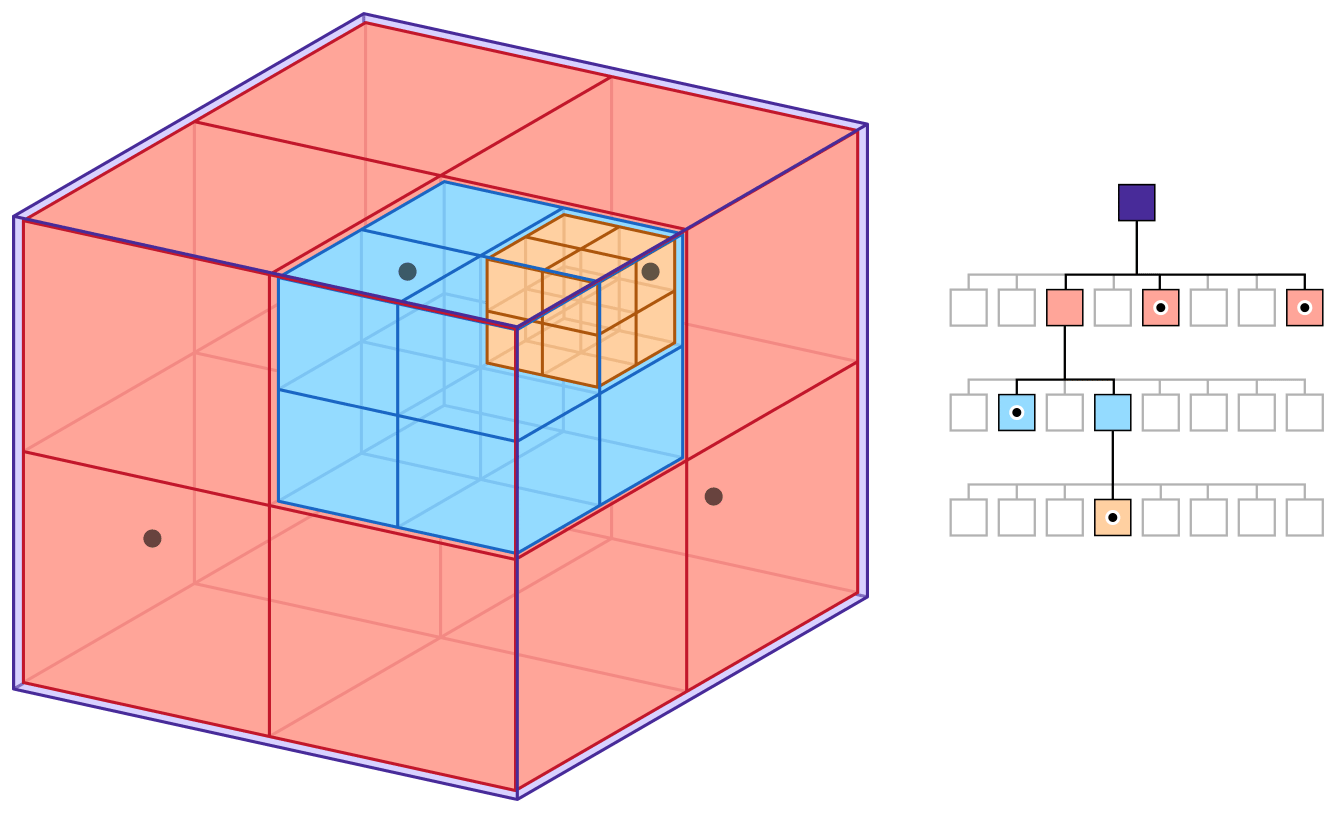
\includegraphics[width=7cm]{figures/octree.png}
\caption{八叉树示意图}
\label{fig:octree}
\end{minipage}
\begin{minipage}[t]{0.38\textwidth}
\centering
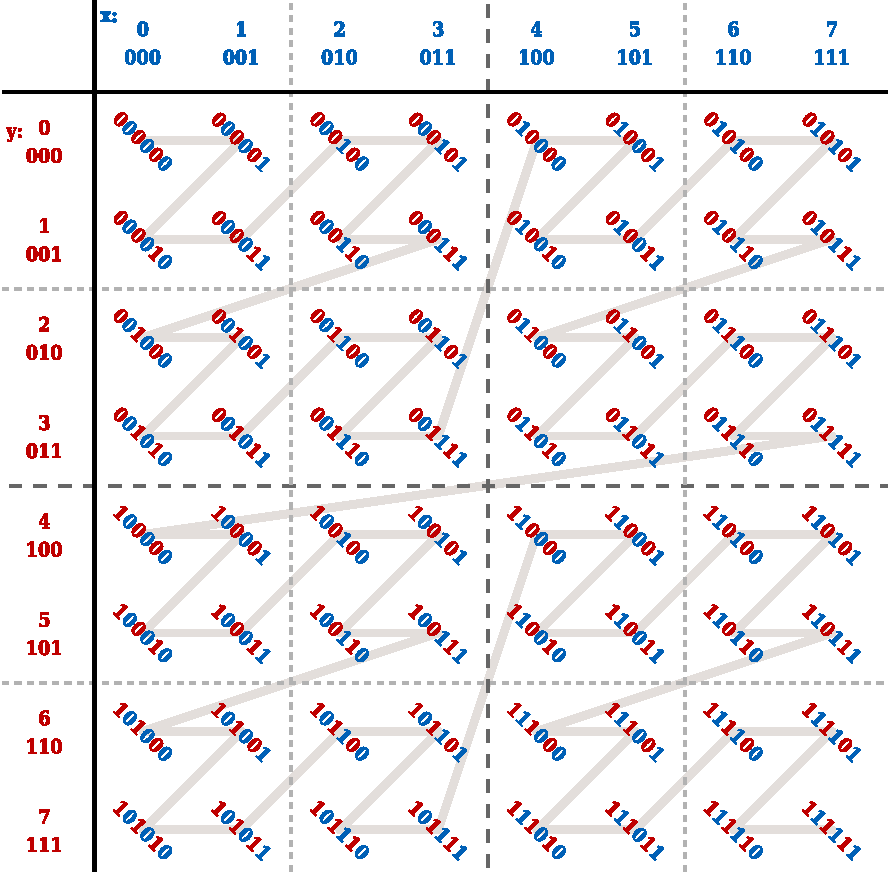
\includegraphics[width=5cm]{figures/Z-curve45.pdf}
\caption{2维情况下的莫顿码编码顺序示意图}
\label{fig:morton_code}
\end{minipage}
\end{figure}

综上,使用莫顿码来对空间的点进行构建八叉树的步骤如下所示:
\begin{enumerate}
    \item 将点的直角坐标转化为莫顿码。
    \item 对莫顿码进行排序。
    \item 逐个比较相邻两个莫顿码的高阶位相等位数,寻找当前点与上一个点在八叉树中的共同祖先节点的深度。
    \item 循环执行第三步,完成八叉树的构建。
\end{enumerate}



\section{八叉树构建硬件加速}

为了更加全面的测试硬件加速性能在不同大小数据集下的表现,我们仍然生成了包含100万、500万和1000万个点的数据集,每组大小的数据集生成三组,共9组数据来进行测试。同时,我们在软件程序当中,对每个步骤进行计时,从而测得不同阶段所花费的时间。我们将建树过程分为三个阶段:编码阶段、排序阶段和建树阶段。根据三个阶段的用时情况以及随着数据集增长而增长的速率,我们就可以得出建树过程中的瓶颈位于哪个阶段。

在这里,我们直接选取相对高效的C语言作为我们的编程语言,同时在莫顿码的排序过程中,我们也采用最高效的16进制基数排序作为排序手段,对三种不同大小的数据集进行测试后,我们得到分阶段的平均用时如表\ref{tab:C_bottleneck}所示。

\begin{table}[htbp]
\centering
\caption{不同大小数据集下使用C语言构建八叉树各阶段平均用时}
\setlength{\tabcolsep}{4mm}{
\begin{tabular}{ccccc}
\toprule
数据集大小    & 编码阶段(ms)      & 排序阶段(ms)     & 建树阶段(ms) & 总用时(ms) \\
\midrule
1000000  & \textbf{223}  & \textbf{45}  & 24       & 292     \\
5000000  & \textbf{1144} & \textbf{252} & 133      & 1529    \\
10000000 & \textbf{2243} & \textbf{479} & 233      & 2955   \\
\bottomrule
\end{tabular}}
\label{tab:C_bottleneck}
\end{table}

根据上面的实验数据,我们不难看出,在这三个阶段当中,编码阶段占用了最多的时间,排序阶段也占用了相当的一部分时间,建树阶段占用的时间最少。因此,我们在设计硬件加速器的过程中,主要关注编码阶段以及排序阶段。对于排序阶段而言,我们也采用之前验证过的最高效的架构——16进制基数排序+传统64路归并排序架构来进行排序。

对于编码阶段来说,其算法中包含了大量的移位操作以及逻辑运算,因此十分适合硬件加速。在编写HLS代码当中,我们在循环中插入了\verb|#pragma HLS pipeline|操作,实现了II=1的流水线架构,从而大大减少了延迟。

我们对我们的硬件架构进行了测试,测试的结果如表\ref{tab:hardware_octree}所示。为了能够更加直观地对比,我们将软件测试结果和硬件测试结果以柱状图形式汇出,如图\ref{fig:Octree_comparison}所示。

\begin{table}[htbp]
\centering
\caption{不同大小数据集下使用硬件加速加速器构建八叉树各阶段用时}
\resizebox{\linewidth}{!}{
\begin{tabular}{cccccc}
\toprule
数据集大小    & 工作频率(MHz) & 编码阶段(ms)       & 排序阶段(ms)       & 建树阶段(同软件)(ms) & 总用时(ms) \\
\midrule
1000000  & 219.3     & \textbf{4.56}  & \textbf{9.69}  & 24            & 38.25   \\
5000000  & 218.25    & \textbf{22.91} & \textbf{48.68} & 133           & 204.59  \\
10000000 & 217.96    & \textbf{45.88} & \textbf{97.5}  & 233           & 376.38 \\
\bottomrule
\end{tabular}}
\label{tab:hardware_octree}
\end{table}

\begin{figure}[htbp]
    \centering
    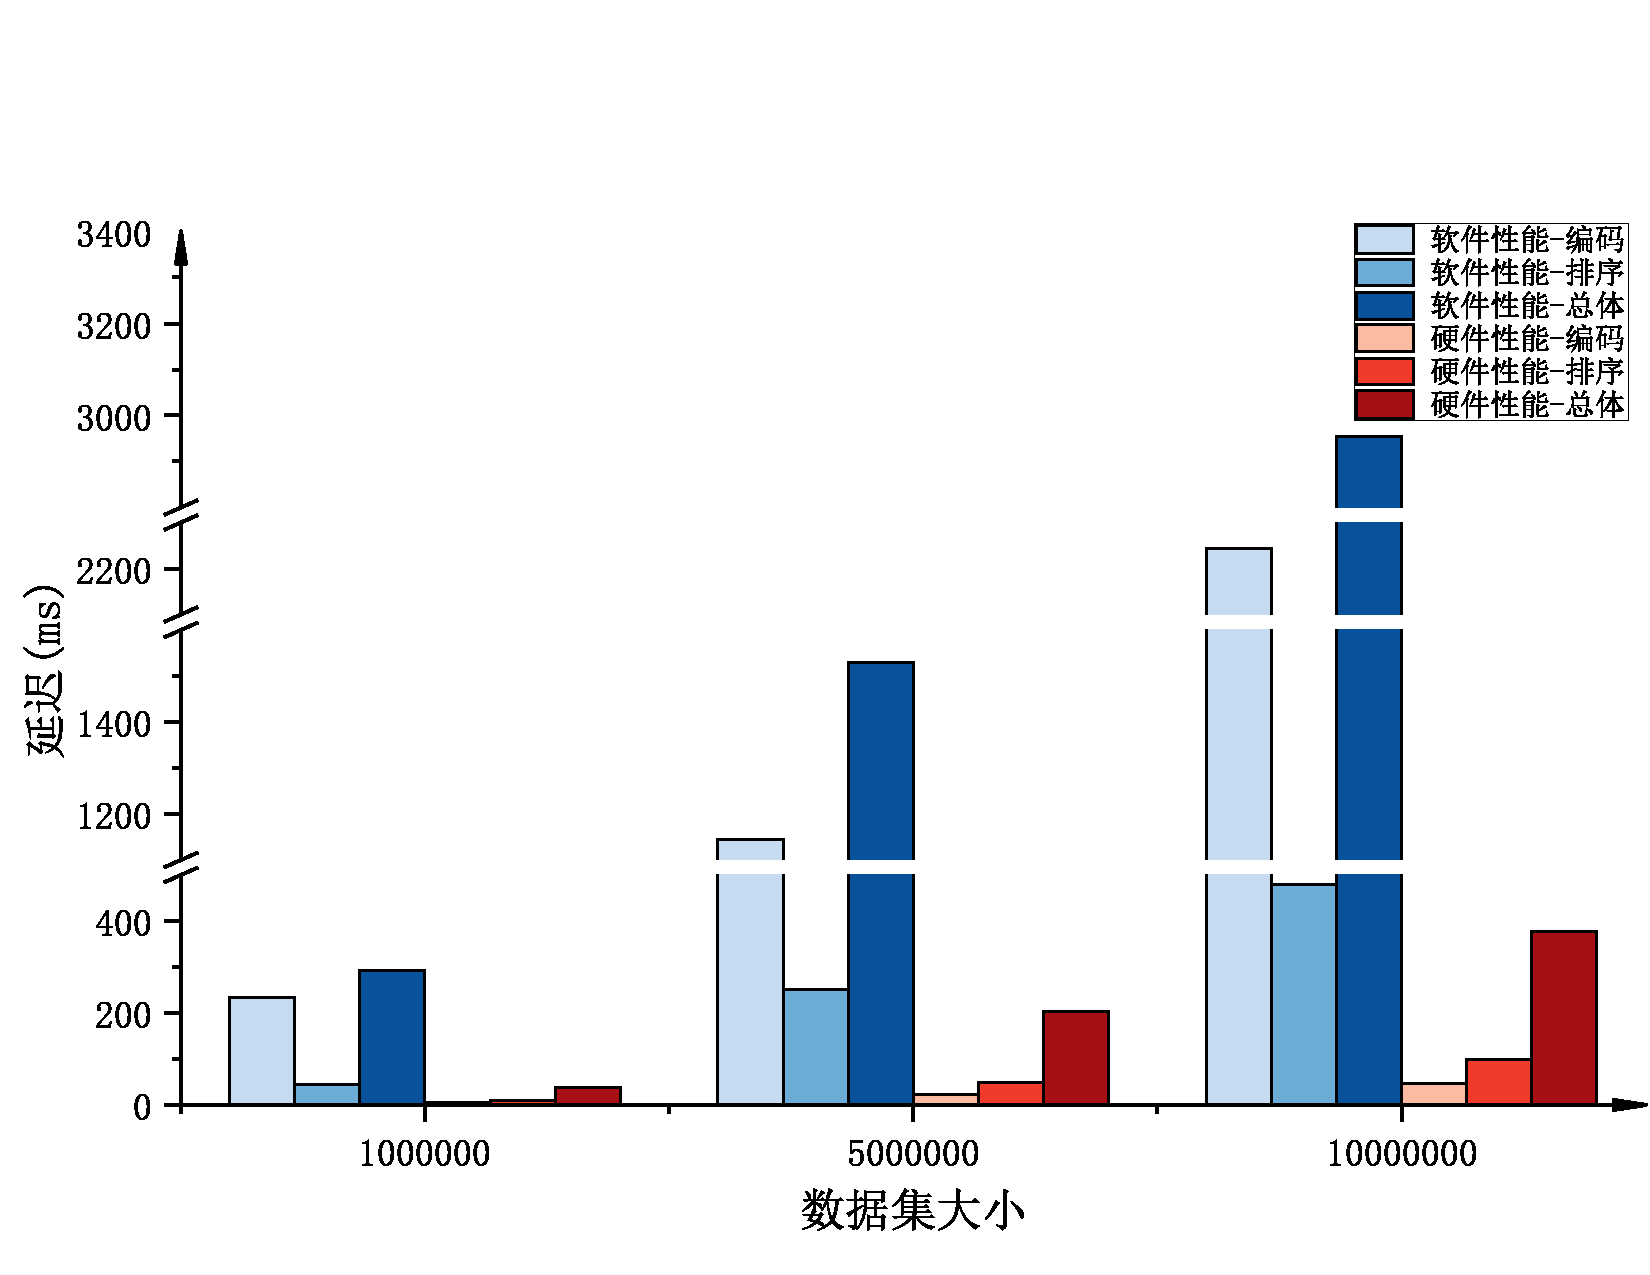
\includegraphics[width=\linewidth]{figures/Octree.pdf}
    \caption{在不同大小数据集下硬件性能与软件性能的对比图}
    \label{fig:Octree_comparison}
\end{figure}


由上可见,采用我们设计的硬件加速器以后,建树效率大大提升,相较于软件算法而言,我们的硬件加速算法能够让全过程耗时减少约87\%,特别是对于软件算法性能的瓶颈——编码和排序阶段,加速效果尤为显著。由此可见,经过搜索空间的选择以及针对性的优化以后,我们给出的硬件加速器是非常高效的,可以用于解决实际问题。

